
\subsubsection{11.11.14}

\begin{enumerate} 
	\item Time of beginning and ending of meeting:
	17:00 - 20:30
	\item Purposes of meeting:
	\begin{enumerate}
		\item To finish MCB.
		
		\item To add to programme of control of robot control of MCB.
		
		\item To write the programme of control of robot with two joysticks.
		
	\end{enumerate}
	
	\item Work that has been done:
	\begin{enumerate}
		\item MCB was finished.
		
		\begin{figure}[H]
			\begin{minipage}[h]{0.47\linewidth}
				\center{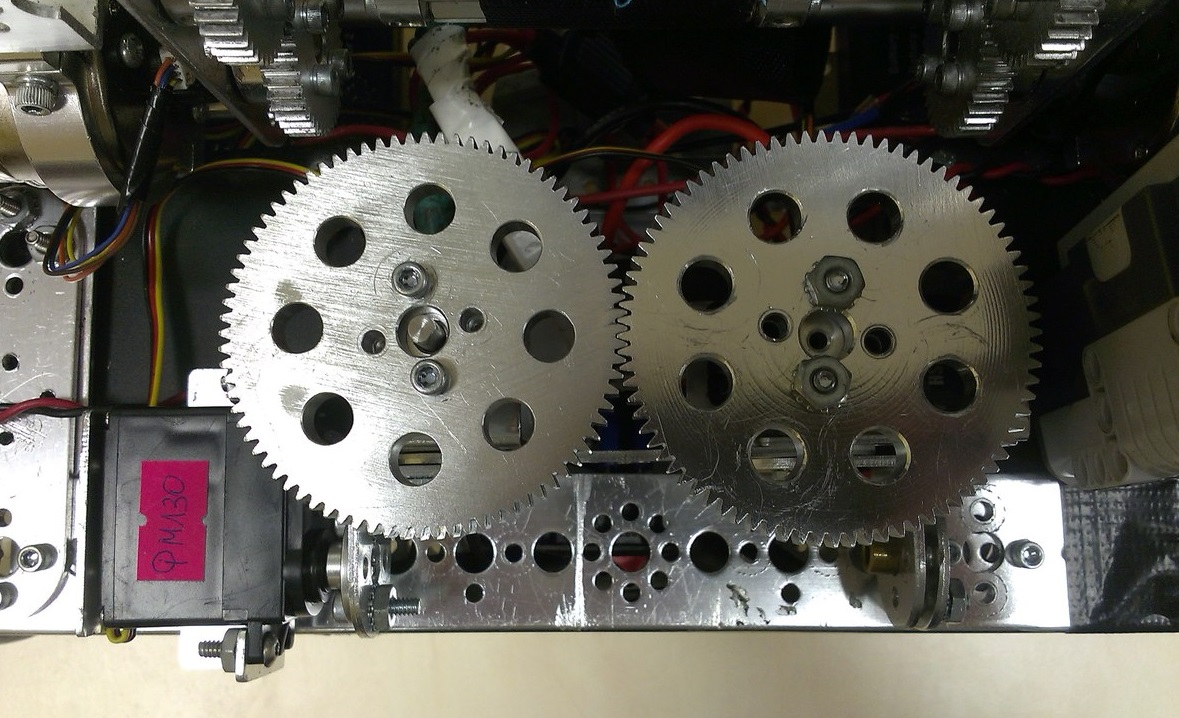
\includegraphics[scale=0.2]{days/11.11.14/images/01}}  
			\end{minipage}
			\begin{minipage}[h]{0.47\linewidth}
				\center{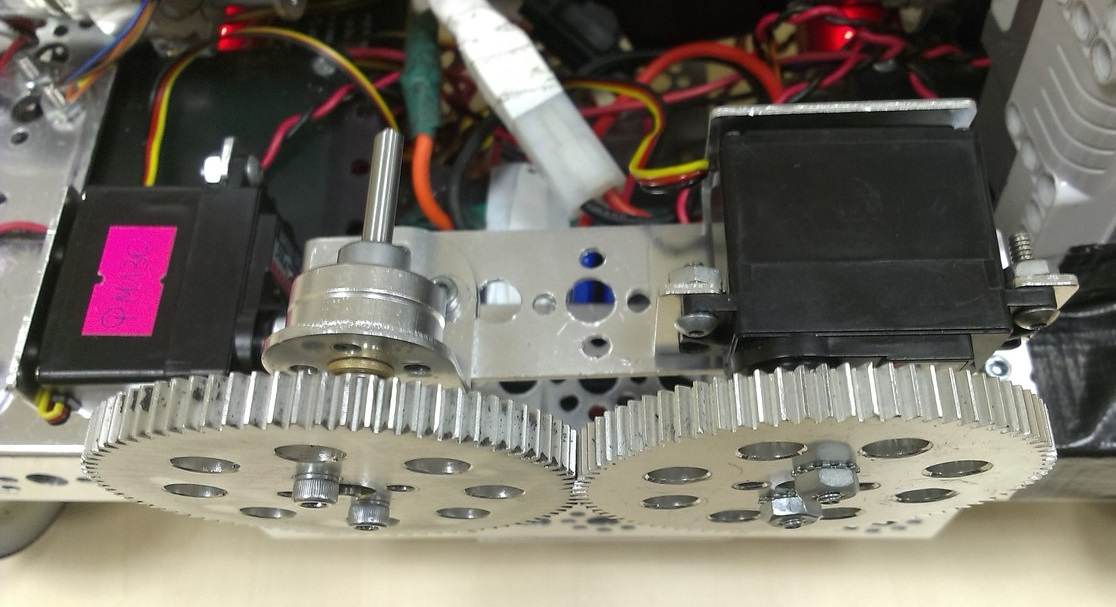
\includegraphics[scale=0.2]{days/11.11.14/images/02}}
			\end{minipage}
			\caption{Finished MCB}
		\end{figure}
		
		\item Programme of control MCB is not implemented.
		
		\item Today it was chosen the place for NXT. Now it was fixed by scotch but we planned to fix it more reliable.
		
		\begin{figure}[H]
			\begin{minipage}[h]{0.2\linewidth}
				\center  
			\end{minipage}
			\begin{minipage}[h]{0.6\linewidth}
				\center{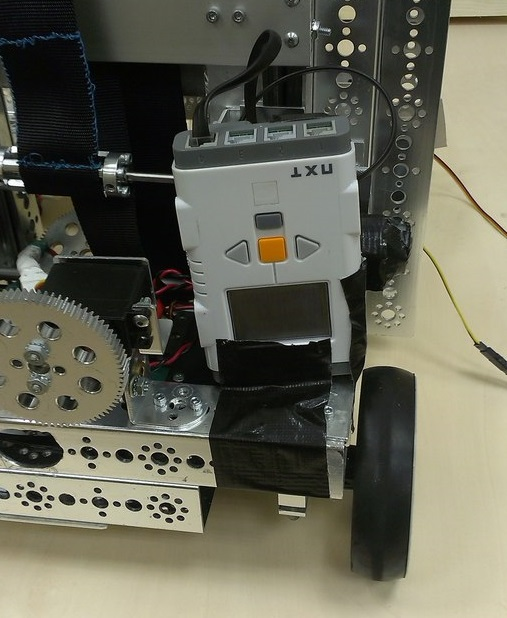
\includegraphics[scale=0.3]{days/11.11.14/images/03}}
				\caption{Place for mount of NXT}
			\end{minipage}
		\end{figure}
		
		\item We noticed that the wire of servo that overturns the bucket touches the floor when lift is folded. It can to prevent of bucket's moving. It was decided to create special coil that works as the roulette and uncoil wire when it is not in tension or fix the wire in several places at the guides of lift.
		
		\item It was decided to create a special programme which allows to us control one of the nodes of robot by NXT's buttons without control with joystick because we often needs to test some one node.
		
		\item The programme of control with two joysticks was created but wasn't tested. In the new programme the first operator responsible for everything except moving and the second responsible for moving.
		
		\item It was elaborated the mechanism of the churning stops and releasing balls in autonomous period: servo of continuous rotation at which will fixed two chains of beams from set Lego-NXT. Every two beams connected by one pin. When it folded this construction doesn't take up much space. When servo starts rotation it will be straight. So for churning stops it will enough to get in the distance of action mechanism. It more easy than write programme of finding stop by IR sensor.
		
		\begin{figure}[H]
			\begin{minipage}[h]{0.2\linewidth}
				\center  
			\end{minipage}
			\begin{minipage}[h]{0.6\linewidth}
				\center{
\includegraphics[scale=0.2]{days/11.11.14/images/04}}
				\caption{Idea of mechanism of churing the stop}
			\end{minipage}
		\end{figure}
		
	\end{enumerate}
	
	\item Results:  
	\begin{enumerate}
		\item MCB was almost finished.
		
		\item Programme of control MCB wasn't implemented.
		
		\item Programme of control robot with two joysticks was created.
		
		\item NXT was fixed at the robot.
		
		\item It was elaborated concept of mechanism of churing of the stops.
		
	\end{enumerate}
	
	\item Tasks for the next meetings:
	\begin{enumerate}
		\item To test programme of control robot with two joysticks.
		
		\item To include to the programme of control robot  the control MCB.
		
		\item To fix the wire of servo, that turn bucket (hereinafter it will call STB) so that it doesn't prevent to moving of lift and bucket.
		
		\item To make the programme of control nodes of robot by buttons of NXT.
		
		\item To create and test the mechanism of churing of the stop.
		
	\end{enumerate}     
\end{enumerate}
\fillpage

